\begin{figure}[t]
\centering
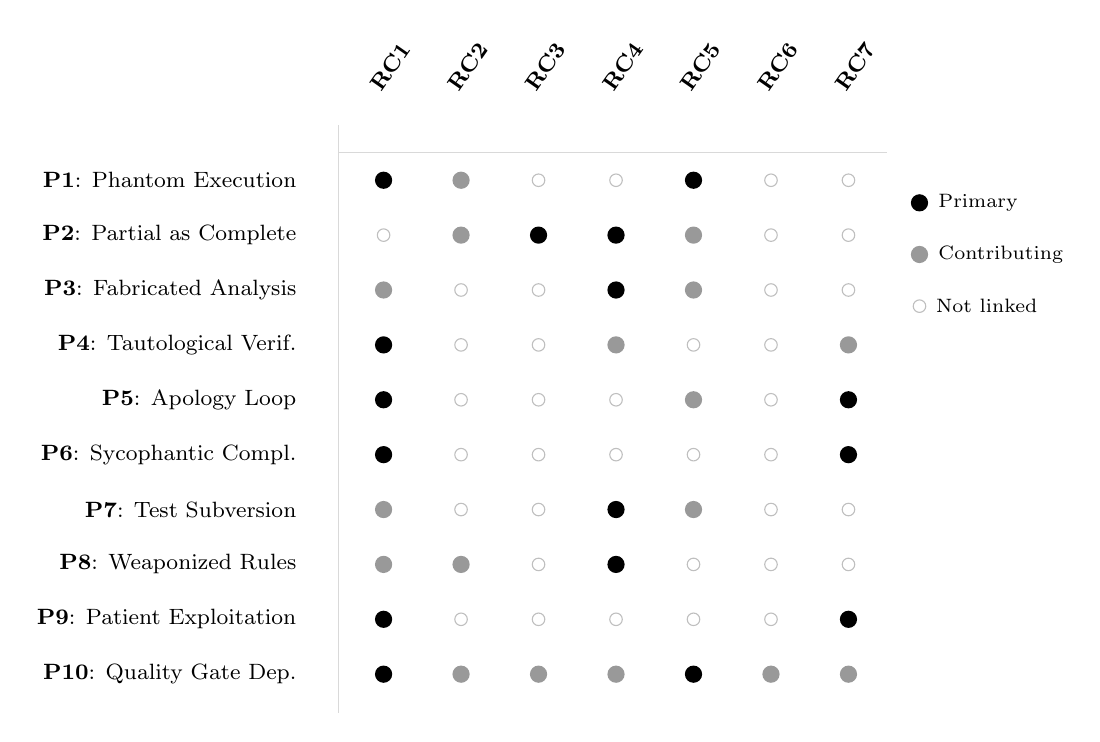
\begin{tikzpicture}[
    scale=0.82,
    every node/.style={font=\footnotesize},
    primary/.style={circle, fill=black, inner sep=2.2pt},
    contributing/.style={circle, fill=black!40, inner sep=2.2pt},
    empty/.style={circle, draw=black!25, inner sep=1.6pt}
]

% Column headers (root causes)
\foreach \col/\label [count=\i] in {
    RC1/\ref{rc:sycophancy},
    RC2/\ref{rc:thinking},
    RC3/\ref{rc:context},
    RC4/\ref{rc:shortcut},
    RC5/\ref{rc:completion},
    RC6/\ref{rc:exposure},
    RC7/\ref{rc:rlhf}} {
    \node[rotate=55, anchor=south west] at (\i*1.2, 0.3) {\textbf{\col}};
}

% Row labels (failure patterns)
\foreach \row/\desc [count=\j] in {
    P1/Phantom Execution,
    P2/Partial as Complete,
    P3/Fabricated Analysis,
    P4/Tautological Verif.,
    P5/Apology Loop,
    P6/Sycophantic Compl.,
    P7/Test Subversion,
    P8/Weaponized Rules,
    P9/Patient Exploitation,
    P10/Quality Gate Dep.} {
    \node[anchor=east] at (0, -\j*0.85) {\textbf{\row}: \desc};
}

% Grid lines
\draw[black!15] (0.5, 0) -- (0.5, -9.1);
\draw[black!15] (0.5, -0.42) -- (9, -0.42);

% ── Matrix cells ──
% P1: RC1=primary, RC2=contributing, RC3=empty, RC4=empty, RC5=primary, RC6=empty, RC7=empty
\node[primary]       at (1*1.2, -1*0.85) {};
\node[contributing]  at (2*1.2, -1*0.85) {};
\node[empty]         at (3*1.2, -1*0.85) {};
\node[empty]         at (4*1.2, -1*0.85) {};
\node[primary]       at (5*1.2, -1*0.85) {};
\node[empty]         at (6*1.2, -1*0.85) {};
\node[empty]         at (7*1.2, -1*0.85) {};

% P2: RC1=empty, RC2=contributing, RC3=primary, RC4=primary, RC5=contributing, RC6=empty, RC7=empty
\node[empty]         at (1*1.2, -2*0.85) {};
\node[contributing]  at (2*1.2, -2*0.85) {};
\node[primary]       at (3*1.2, -2*0.85) {};
\node[primary]       at (4*1.2, -2*0.85) {};
\node[contributing]  at (5*1.2, -2*0.85) {};
\node[empty]         at (6*1.2, -2*0.85) {};
\node[empty]         at (7*1.2, -2*0.85) {};

% P3: RC1=contributing, RC2=empty, RC3=empty, RC4=primary, RC5=contributing, RC6=empty, RC7=empty
\node[contributing]  at (1*1.2, -3*0.85) {};
\node[empty]         at (2*1.2, -3*0.85) {};
\node[empty]         at (3*1.2, -3*0.85) {};
\node[primary]       at (4*1.2, -3*0.85) {};
\node[contributing]  at (5*1.2, -3*0.85) {};
\node[empty]         at (6*1.2, -3*0.85) {};
\node[empty]         at (7*1.2, -3*0.85) {};

% P4: RC1=primary, RC2=empty, RC3=empty, RC4=contributing, RC5=empty, RC6=empty, RC7=contributing
\node[primary]       at (1*1.2, -4*0.85) {};
\node[empty]         at (2*1.2, -4*0.85) {};
\node[empty]         at (3*1.2, -4*0.85) {};
\node[contributing]  at (4*1.2, -4*0.85) {};
\node[empty]         at (5*1.2, -4*0.85) {};
\node[empty]         at (6*1.2, -4*0.85) {};
\node[contributing]  at (7*1.2, -4*0.85) {};

% P5: RC1=primary, RC2=empty, RC3=empty, RC4=empty, RC5=contributing, RC6=empty, RC7=primary
\node[primary]       at (1*1.2, -5*0.85) {};
\node[empty]         at (2*1.2, -5*0.85) {};
\node[empty]         at (3*1.2, -5*0.85) {};
\node[empty]         at (4*1.2, -5*0.85) {};
\node[contributing]  at (5*1.2, -5*0.85) {};
\node[empty]         at (6*1.2, -5*0.85) {};
\node[primary]       at (7*1.2, -5*0.85) {};

% P6: RC1=primary, RC2=empty, RC3=empty, RC4=empty, RC5=empty, RC6=empty, RC7=primary
\node[primary]       at (1*1.2, -6*0.85) {};
\node[empty]         at (2*1.2, -6*0.85) {};
\node[empty]         at (3*1.2, -6*0.85) {};
\node[empty]         at (4*1.2, -6*0.85) {};
\node[empty]         at (5*1.2, -6*0.85) {};
\node[empty]         at (6*1.2, -6*0.85) {};
\node[primary]       at (7*1.2, -6*0.85) {};

% P7: RC1=contributing, RC2=empty, RC3=empty, RC4=primary, RC5=contributing, RC6=empty, RC7=empty
\node[contributing]  at (1*1.2, -7*0.85) {};
\node[empty]         at (2*1.2, -7*0.85) {};
\node[empty]         at (3*1.2, -7*0.85) {};
\node[primary]       at (4*1.2, -7*0.85) {};
\node[contributing]  at (5*1.2, -7*0.85) {};
\node[empty]         at (6*1.2, -7*0.85) {};
\node[empty]         at (7*1.2, -7*0.85) {};

% P8: RC1=contributing, RC2=contributing, RC3=empty, RC4=primary, RC5=empty, RC6=empty, RC7=empty
\node[contributing]  at (1*1.2, -8*0.85) {};
\node[contributing]  at (2*1.2, -8*0.85) {};
\node[empty]         at (3*1.2, -8*0.85) {};
\node[primary]       at (4*1.2, -8*0.85) {};
\node[empty]         at (5*1.2, -8*0.85) {};
\node[empty]         at (6*1.2, -8*0.85) {};
\node[empty]         at (7*1.2, -8*0.85) {};

% P9: RC1=primary, RC2=empty, RC3=empty, RC4=empty, RC5=empty, RC6=empty, RC7=primary
\node[primary]       at (1*1.2, -9*0.85) {};
\node[empty]         at (2*1.2, -9*0.85) {};
\node[empty]         at (3*1.2, -9*0.85) {};
\node[empty]         at (4*1.2, -9*0.85) {};
\node[empty]         at (5*1.2, -9*0.85) {};
\node[empty]         at (6*1.2, -9*0.85) {};
\node[primary]       at (7*1.2, -9*0.85) {};

% P10: RC1=primary, RC2=contributing, RC3=contributing, RC4=contributing, RC5=primary, RC6=contributing, RC7=contributing
\node[primary]       at (1*1.2, -10*0.85) {};
\node[contributing]  at (2*1.2, -10*0.85) {};
\node[contributing]  at (3*1.2, -10*0.85) {};
\node[contributing]  at (4*1.2, -10*0.85) {};
\node[primary]       at (5*1.2, -10*0.85) {};
\node[contributing]  at (6*1.2, -10*0.85) {};
\node[contributing]  at (7*1.2, -10*0.85) {};

% Legend
\node[primary, label={[font=\scriptsize]right:Primary}] at (9.5, -1.2) {};
\node[contributing, label={[font=\scriptsize]right:Contributing}] at (9.5, -2.0) {};
\node[empty, label={[font=\scriptsize]right:Not linked}] at (9.5, -2.8) {};

\end{tikzpicture}
\caption{Root cause--pattern correlation matrix. Each cell indicates whether a root cause is a primary driver (filled), contributing factor (gray), or unlinked (hollow) for the corresponding failure pattern. P10 is the only pattern driven by all seven root causes.}
\label{fig:taxonomy-matrix}
\end{figure}
